\section{結果}
\label{sec:results}

本節の結果は二つに分かれる。
第一に、\Method と公開実装ベースラインを
同一のアライメント手続きで比較した交差モデル比較であり、
実写 held-out validation と合成 trajectory-group test の
二つの domain で測定済みである。
第二に、checkpoint 選択時に記録された
合成 validation の値であり、
これは同じ条件で比較相手を走らせた測定ではない。
両者を混ぜない。

\subsection{交差モデル比較の条件}
\label{sec:comparison_setup}

比較は固定した manifest に従って一度だけ実行した。
各 domain で決定論的に \resBenchDomainSamples 件（seed \resBenchSeed）を選び、
両モデルへ同じ画像を渡し、
得られた生のキーポイントへ\emph{同一の} RANSAC アライメントを適用する。
したがって検出器の内部構造ではなく、
「検出した点をどれだけ一つの射影幾何へまとめられるか」を比較している。

推論はすべて CPU で行った。
\texttt{CUDA\_VISIBLE\_DEVICES} を空にし、
\texttt{torch.cuda.is\_available()} が偽であることを記録した環境で、
二つの domain と二つのモデルを合わせて \resBenchElapsedSeconds 秒で完了した。
ホモグラフィの RANSAC 閾値は画像対角線の \resBenchRansacThreshold、
線再投影は規制線の各セグメント \resBenchLineSegmentSamples 点サンプルである。

二つの domain の意味は異なる。
\texttt{real\_validation} は公開実装付属データの held-out validation であり、
\emph{公式の test split ではない}。
\texttt{synthetic\_test} は trajectory-group-disjoint な test であり、
同じ会場群の未学習軌道を見る。
未知会場での評価ではない。

\paragraph{可視性の定義}
両 domain で「GT-visible」の定義が異なる。
実写側は注釈が画像内にあることを GT-visible とし、
合成側はカメラ前方・画面内・レンダラが見ているという三条件を満たす点だけを
GT-visible とする。
したがって Complete の絶対値を domain 間で直接比較しない。
domain 内のモデル比較は同じ分母で行う。

\subsection{実写 held-out validation}
\label{sec:results_real}

\cref{tab:court-alignment} の上段に実写の結果を示す。

\begin{table}[t]
  \centering
  \caption{\textbf{交差モデル比較。}
  実写 \texttt{real\_validation} は公開実装付属の held-out validation
  （公式 test ではない）、合成 \texttt{synthetic\_test} は
  trajectory-group-disjoint test（同じ会場群の未学習軌道であり未知会場ではない）。
  両 domain は決定論的に選んだ \resBenchDomainSamples 件（seed \resBenchSeed）である。
  Complete は GT-visible のキーポイントのうちモデルが返したものの割合、
  PCK は画像対角線に対する閾値（@0.01 は 1\%）で、
  返さなかった点は不正解として数える。
  Pair median はモデルが返した点だけの対応誤差の中央値であり、
  括弧内はその pair 数である。
  H success は正準規制テンプレートから画像への共通 RANSAC ホモグラフィの成功率で、
  分母は全 \resBenchDomainSamples 件、失敗も分母に含める。
  IoU 定義/全 は画像でクリップしたダブルス多角形の IoU の中央値と、
  値が定義できた件数/全件数であり、
  縮退した多角形は値を持たないため定義件数を併記する。
  domain を跨いだ Complete の絶対値は直接比較しない。
  }
  \label{tab:court-alignment}
  \footnotesize
  \setlength{\tabcolsep}{4pt}
  \begin{tabular}{@{}llrrrrrr@{}}
    \toprule
    Domain & Model & Complete & @0.01 & @0.02 &
      Pair med. (px) & H succ. & IoU 定義/全 \\
    \midrule
    \texttt{real\_validation} & ours &
      \resRealOursComplete & \resRealOursPckOne & \resRealOursPckTwo &
      \resRealOursPairMedian\ (\resRealOursPairN) &
      \resRealOursHSuccessCount & \resRealOursIouMedian\ (\resRealOursIouDefined/\resRealOursIouTotal) \\
    \texttt{real\_validation} & TCD &
      \resRealTcdComplete & \resRealTcdPckOne & \resRealTcdPckTwo &
      \resRealTcdPairMedian\ (\resRealTcdPairN) &
      \resRealTcdHSuccessCount & \resRealTcdIouMedian\ (\resRealTcdIouDefined/\resRealTcdIouTotal) \\
    \midrule
    \texttt{synthetic\_test} & ours &
      \resSynthOursComplete & \resSynthOursPckOne & \resSynthOursPckTwo &
      \resSynthOursPairMedian\ (\resSynthOursPairN) &
      \resSynthOursHSuccessCount & \resSynthOursIouMedian\ (\resSynthOursIouDefined/\resSynthOursIouTotal) \\
    \texttt{synthetic\_test} & TCD &
      \resSynthTcdComplete & \resSynthTcdPckOne & \resSynthTcdPckTwo &
      \resSynthTcdPairMedian\ (\resSynthTcdPairN) &
      \resSynthTcdHSuccessCount &
      \resNotApplicable\ (\resSynthTcdIouDefined/\resSynthTcdIouTotal) \\
    \bottomrule
  \end{tabular}
\end{table}


\Method は GT-visible \resRealOursVisible 点のすべてを返し、
Complete は \resRealOursComplete である。
対応誤差は中央値 \resRealOursPairMedian px、
平均 \resRealOursPairMean px、q90 \resRealOursPairQ px で、
PCK@0.01 は \resRealOursPckOne である。
共通 RANSAC は \resRealOursHSuccessCount 件すべてで成功した。

\BaselineShort も Complete \resRealTcdComplete、
PCK@0.01 \resRealTcdPckOne、RANSAC 成功 \resRealTcdHSuccessCount と健闘する。
差がはっきり出るのは PCK@0.005（\resRealOursPckHalf 対 \resRealTcdPckHalf）と
対応誤差の平均（\resRealOursPairMean px 対 \resRealTcdPairMean px）である。
実写 held-out validation では \Method が僅かに上回るが、
この差は「大差」と呼べるものではない。

線再投影の平均には注意が要る。
\BaselineShort の画面内平均は \resRealTcdLineInMean px と大きく出るが、
中央値は \resRealTcdLineInMedian px、q90 は \resRealTcdLineInQ px である。
内訳を見ると、GT-visible が \resRealTcdOutlierVisible 点しかない 1 標本で
\BaselineShort が 5 点しか返さず、
その 1 標本がおよそ \resRealTcdOutlierPx px の外れ値になり平均を押し上げている。
平均だけを報告すれば、この標本の寄与が見えなくなる。

\cref{fig:summary_bars} に主要指標を、
\cref{fig:montage_real} に実写の代表例を示す。

\begin{figure}[t]
  \centering
  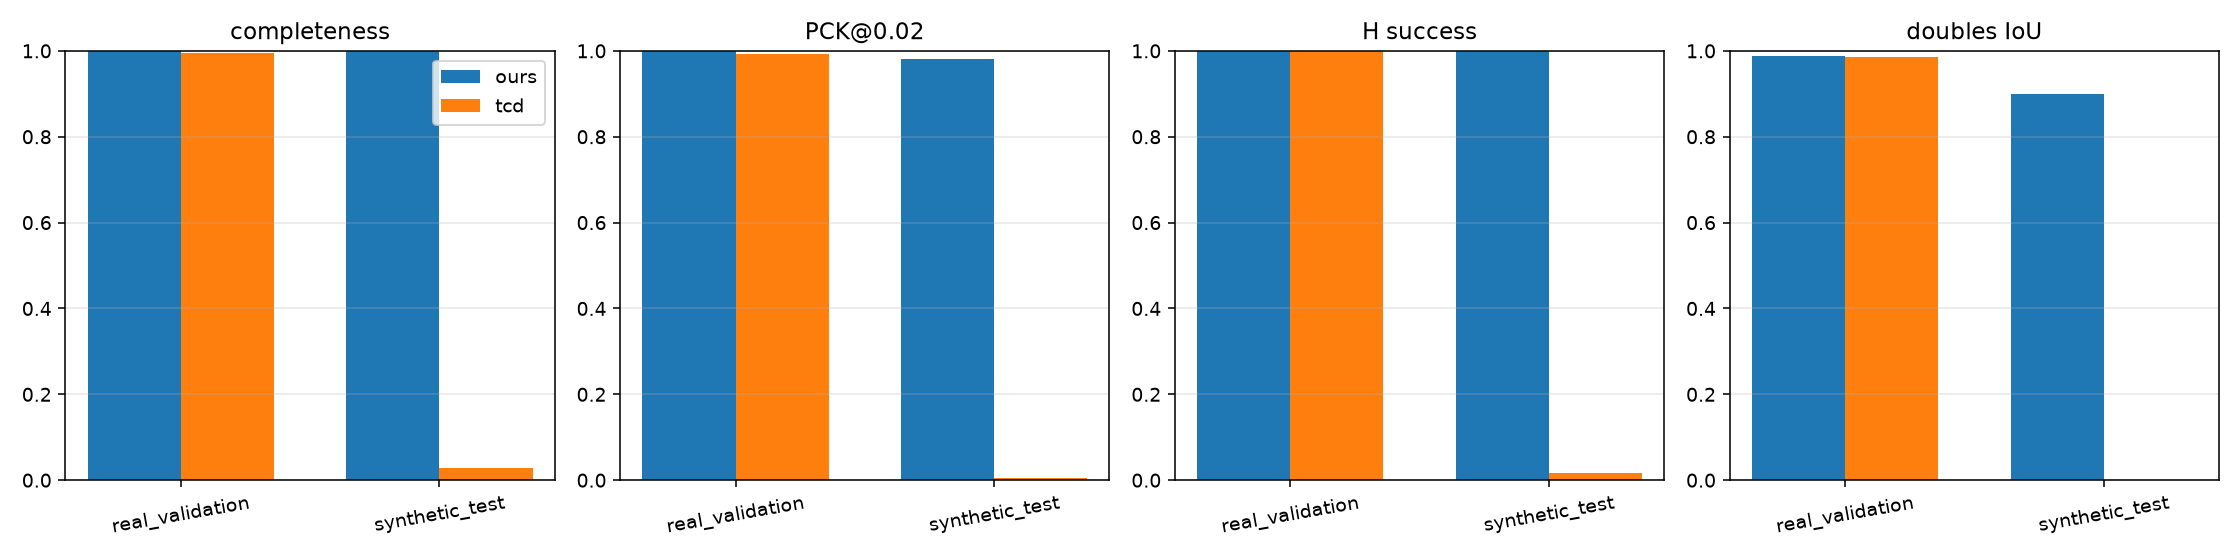
\includegraphics[width=\linewidth]{figures/generated/summary_bars.png}
  \caption{\textbf{交差モデル比較の主要指標。}
  \resBenchDomainSamples 件ずつの決定論的標本（seed \resBenchSeed）。
  Complete と PCK@0.02 は返さなかったキーポイントを不正解として数えた値であり、
  H success も失敗を分母に含めた成功率である。
  したがって棒が無い区間は「0 に近い」ことを示し、
  値が定義されない区間（合成のダブルス IoU）は棒を描かずに省略している。
  domain を跨いだ Complete の絶対値は定義が違うため直接比較しない。
  }
  \label{fig:summary_bars}
\end{figure}

\begin{figure}[t]
  \centering
  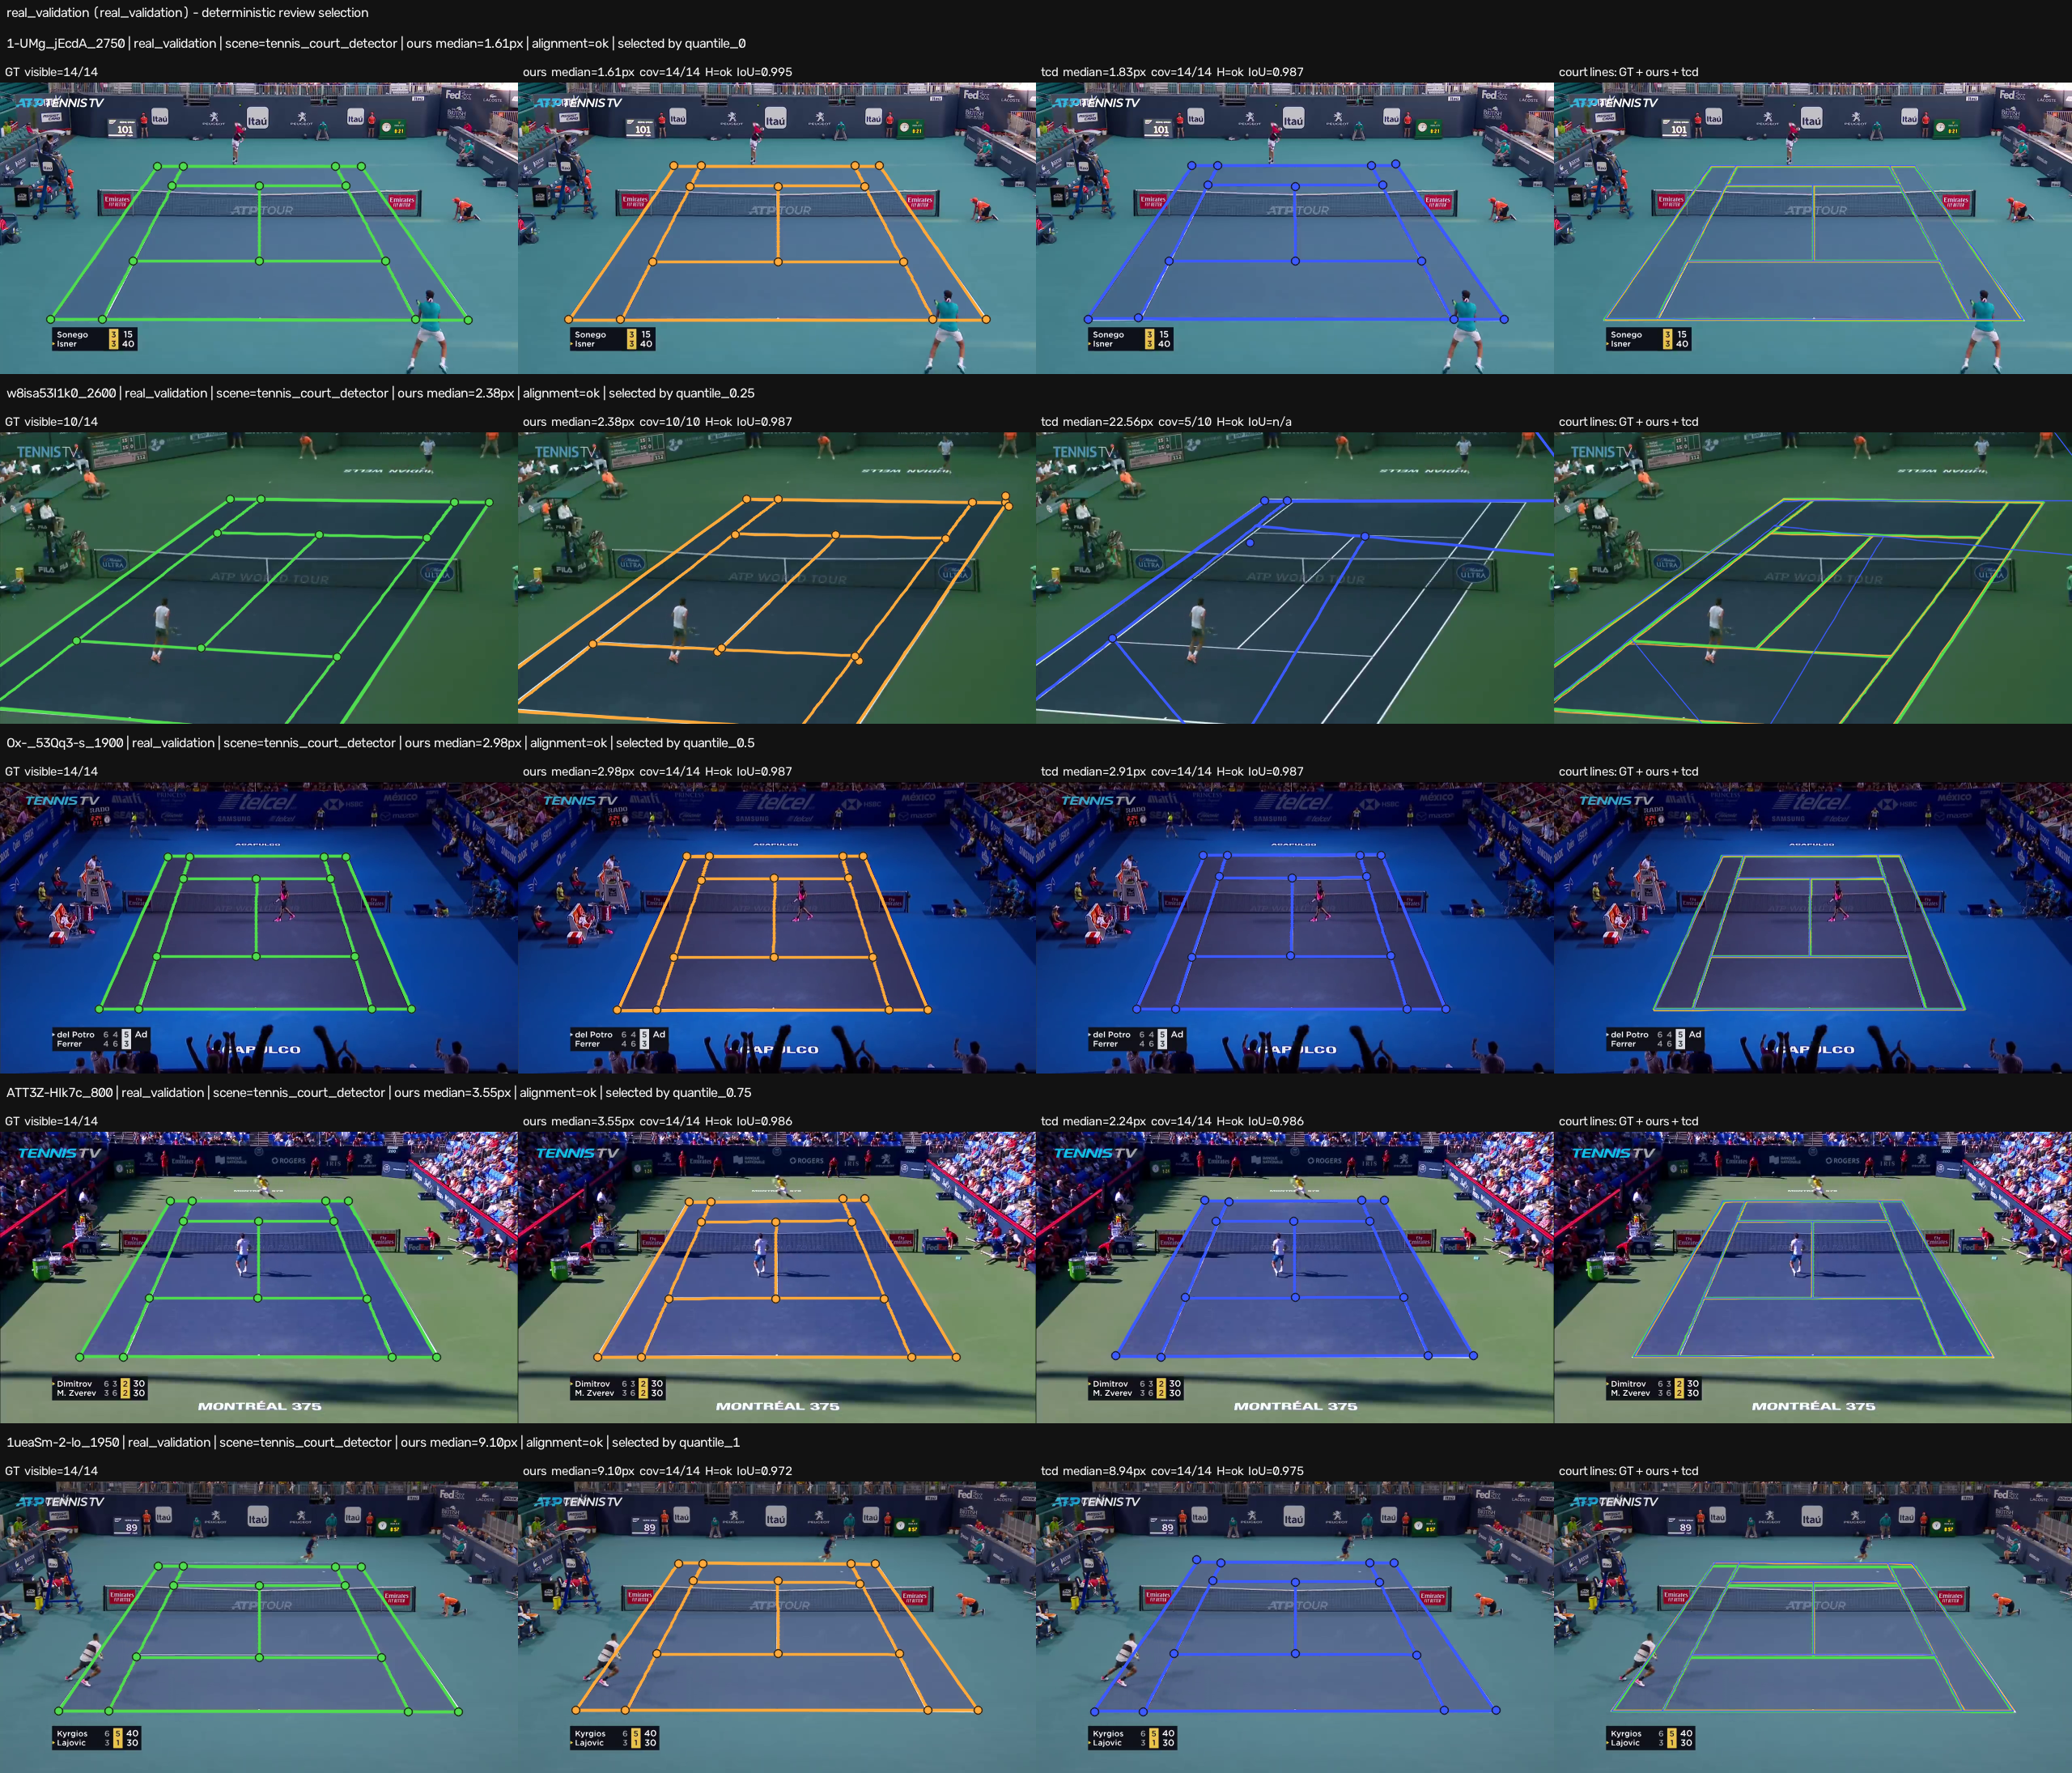
\includegraphics[width=\linewidth]{figures/generated/montage_real_validation.png}
  \caption{\textbf{実写 held-out validation の代表例。}
  誤差の分位点（quantile 0, 0.25, 0.5, 0.75, 1）で
  決定論的に選んだ 5 例である。
  緑は GT、橙は \Method、青は \BaselineShort。
  4 列目は重畳で、二つのモデルの一致と食い違いが見える。
  下段に行くほど対応誤差が大きい。
  }
  \label{fig:montage_real}
\end{figure}

\subsection{合成 trajectory-group test}
\label{sec:results_synthetic}

\cref{tab:court-alignment} の下段に合成 test の結果を示す。

\Method は GT-visible \resSynthOursVisible 点をすべて返し、
Complete \resSynthOursComplete、PCK@0.01 \resSynthOursPckOne、
PCK@0.02 \resSynthOursPckTwo である。
対応誤差は中央値 \resSynthOursPairMedian px、平均 \resSynthOursPairMean px、
q90 \resSynthOursPairQ px で、平均と中央値の開きが
視点条件の悪い標本の重い裾を示す。
共通 RANSAC は \resSynthOursHSuccessCount 件ですべて成功した。

\BaselineShort は同じ test でほぼ機能しない。
Complete は \resSynthTcdComplete、PCK@0.01 は \resSynthTcdPckOne であり、
有効な対応が得られたのは \resSynthTcdPairN 点だけである。
RANSAC 成功は \resSynthTcdHSuccessCount 件にとどまり、
失敗の内訳は有効キーポイント不足が \resSynthTcdInsufficientFailures 件、
RANSAC 自体の失敗が \resSynthTcdRansacFailures 件である。
ダブルス多角形 IoU は \resSynthTcdIouDefined/\resSynthTcdIouTotal 件でしか定義できなかった。
予測ホモグラフィが得られなかった 118 件は IoU 計算へ進めず、
ホモグラフィが得られた 2 件も画像でクリップ後の多角形が縮退した。
会場別に見ると \resSynthTcdSceneBzeroN 件の \texttt{B00} だけが
Complete \resSynthTcdSceneBzeroComplete、RANSAC 成功 \resSynthTcdSceneBzeroHSuccess 件を出し、
他の会場は有効検出が \resSynthTcdSceneOtherValid 件である。

この結果は「\BaselineShort の学習分布に合成データが無い」という仮説と整合する。
ただし両者のアーキテクチャと学習データは同時に異なるため、
本稿はこれを原因として断定しない。

\begin{table}[t]
  \centering
  \caption{\textbf{合成 test を撮影範囲の被覆率で層別した内訳（ours）。}
  層は GT のコート線サンプルのうち画像内に落ちる割合で分けた。
  \texttt{full} はコート全体、\texttt{near\_full} はほぼ全体、
  \texttt{partial} は一部だけが画面内に入る。
  coverage の低い層ほど誤差の裾が伸びるが、
  どの層でも PCK@0.01 は 0.92 を下回らない。
  }
  \label{tab:comparison_strata}
  \small
  \begin{tabular}{@{}lrrrr@{}}
    \toprule
    層 & \(n\) & 画面内線 median (px) & PCK@0.01 & GT-visible 点 \\
    \midrule
    \texttt{full} & \resSynthOursFullN &
      \resSynthOursFullLineMedian & \resSynthOursFullPckOne & \resSynthOursFullVisible \\
    \texttt{near\_full} & \resSynthOursNearFullN &
      \resSynthOursNearFullLineMedian & \resSynthOursNearFullPckOne & \resSynthOursNearFullVisible \\
    \texttt{partial} & \resSynthOursPartialN &
      \resSynthOursPartialLineMedian & \resSynthOursPartialPckOne & \resSynthOursPartialVisible \\
    \bottomrule
  \end{tabular}
\end{table}

\begin{table}[t]
  \centering
  \caption{\textbf{合成 test の会場別 PCK@0.01（ours）。}
  test は trajectory-group-disjoint であり、
  会場自体は学習にも現れる。したがってこの表は
  未知会場への汎化ではなく、
  同じ会場の未学習軌道でのばらつきを示す。
  }
  \label{tab:comparison_scene}
  \small
  \begin{tabular}{@{}lrr@{}}
    \toprule
    会場 & \(n\) & PCK@0.01 \\
    \midrule
    \texttt{B00} & \resSynthOursSceneBzeroN & \resSynthOursSceneBzeroPckOne \\
    \texttt{B01} & \resSynthOursSceneBoneN & \resSynthOursSceneBonePckOne \\
    \texttt{B02} & \resSynthOursSceneBtwoN & \resSynthOursSceneBtwoPckOne \\
    \texttt{B03} & \resSynthOursSceneBthreeN & \resSynthOursSceneBthreePckOne \\
    \bottomrule
  \end{tabular}
\end{table}


合成側の誤差は撮影範囲の被覆率に強く依存する。
\cref{tab:comparison_strata} のとおり、
コート全体が画面に入る層では画面内線誤差の中央値が
\resSynthOursFullLineMedian px であるのに対し、
一部だけが入る層では \resSynthOursPartialLineMedian px になる。
PCK@0.01 は層を通じて 0.92 以上を保つ。
会場別の PCK@0.01 は \cref{tab:comparison_scene} に示す。

\begin{figure}[t]
  \centering
  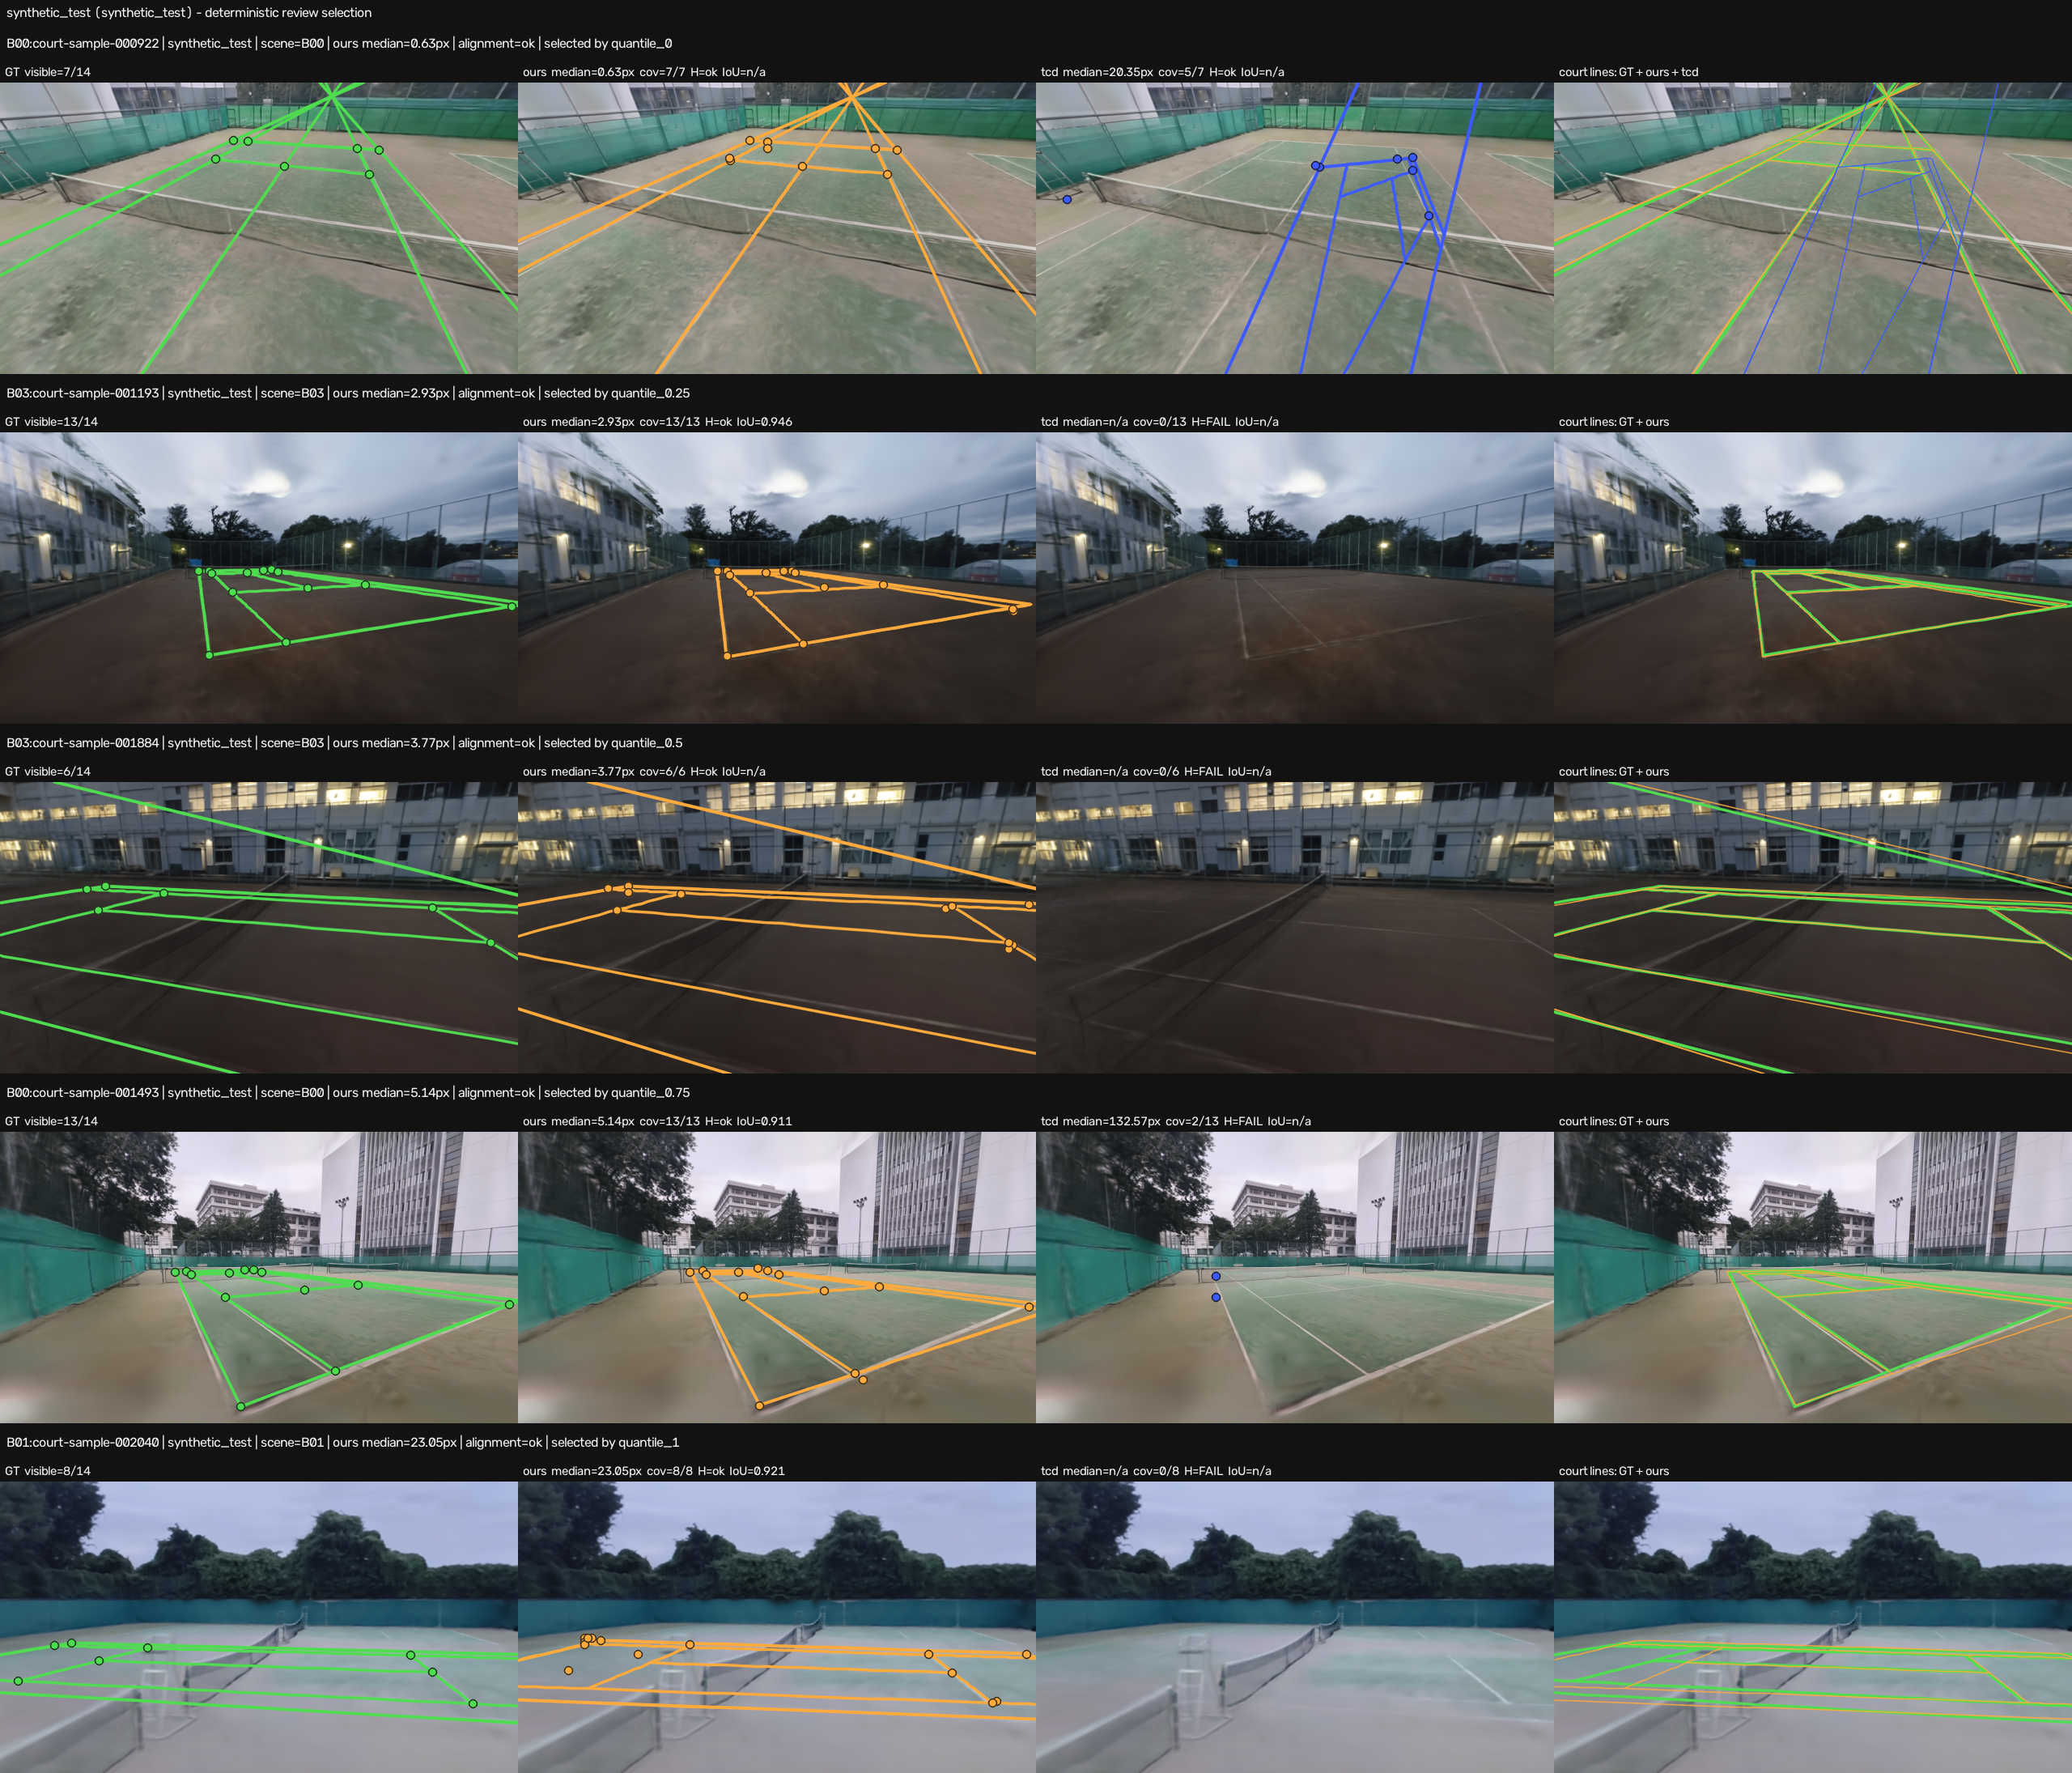
\includegraphics[width=\linewidth]{figures/generated/montage_synthetic_test.png}
  \caption{\textbf{合成 trajectory-group test の代表例。}
  誤差の分位点（quantile 0, 0.25, 0.5, 0.75, 1）で
  決定論的に選んだ 5 例である。
  緑は GT、橙は \Method、青は \BaselineShort。
  \BaselineShort は多くの例でコートを支持する点を出せず、
  4 列目の重畳でも橙だけが残る。
  最後の 2 例は撮影範囲が部分的で、
  コートの一部だけが画面内に入る条件である。
  }
  \label{fig:montage_synthetic}
\end{figure}

\subsection{設計した指標の内訳}
\label{sec:results_metrics}

\cref{tab:keypoint_detail} に閾値掃引と対応誤差の裾を、
\cref{tab:line_detail} に線再投影の全標本と画面内標本を示す。

\begin{table}[t]
  \centering
  \caption{\textbf{キーポイント指標の閾値掃引と対応誤差の分布。}
  PCK は画像対角線に対する閾値で、返さなかったキーポイントは不正解として数える。
  対応誤差の統計はモデルが返した点だけを対象にし、
  pair 数 \(n\) を併記する（モデル間で \(n\) が異なる）。
  }
  \label{tab:keypoint_detail}
  \footnotesize
  \setlength{\tabcolsep}{4pt}
  \begin{tabular}{@{}llrrrrrrr@{}}
    \toprule
    Domain & Model & @0.005 & @0.01 & @0.02 & @0.05 &
      \(n\) & Pair med. (px) \\
    \midrule
    \texttt{real\_validation} & ours &
      \resRealOursPckHalf & \resRealOursPckOne & \resRealOursPckTwo & --- &
      \resRealOursPairN & \resRealOursPairMedian \\
    \texttt{real\_validation} & TCD &
      \resRealTcdPckHalf & \resRealTcdPckOne & \resRealTcdPckTwo & --- &
      \resRealTcdPairN & \resRealTcdPairMedian \\
    \midrule
    \texttt{synthetic\_test} & ours &
      \resSynthOursPckHalf & \resSynthOursPckOne & \resSynthOursPckTwo & \resSynthOursPckFive &
      \resSynthOursPairN & \resSynthOursPairMedian \\
    \texttt{synthetic\_test} & TCD &
      \resSynthTcdPckHalf & \resSynthTcdPckOne & \resSynthTcdPckTwo & \resSynthTcdPckFive &
      \resSynthTcdPairN & \resSynthTcdPairMedian \\
    \bottomrule
  \end{tabular}
\end{table}

\begin{table}[t]
  \centering
  \caption{\textbf{線再投影誤差の全標本と画面内標本。}
  規制線を各セグメント \resBenchLineSegmentSamples 点でサンプルし、
  モデルのホモグラフィと GT ホモグラフィの対称再投影誤差を測る。
  「全サンプル」は画面外へ外挿したサンプルを含むため、
  合成側では桁が変わりうる（\cref{sec:results_metrics} を参照）。
  「画面内」は GT の投影が画像内に落ちるサンプルだけの集計であり、
  画面内率はその割合である。
  }
  \label{tab:line_detail}
  \footnotesize
  \setlength{\tabcolsep}{4pt}
  \begin{tabular}{@{}llrrrrr@{}}
    \toprule
    Domain & Model &
      全 med. (px) &
      画面内 mean & 画面内 med. & 画面内 q90 & 画面内率 \\
    \midrule
    \texttt{real\_validation} & ours &
      \resRealOursLineMedian &
      \resRealOursLineInMean & \resRealOursLineInMedian &
      \resRealOursLineInQ & \resRealOursLineInFraction \\
    \texttt{real\_validation} & TCD &
      \resRealTcdLineMedian &
      \resRealTcdLineInMean & \resRealTcdLineInMedian &
      \resRealTcdLineInQ & \resRealTcdLineInFraction \\
    \midrule
    \texttt{synthetic\_test} & ours &
      \resSynthOursLineMedian &
      \resSynthOursLineInMean & \resSynthOursLineInMedian &
      \resSynthOursLineInQ & \resSynthOursLineInFraction \\
    \texttt{synthetic\_test} & TCD &
      \resSynthTcdLineMedian &
      \resSynthTcdLineInMean & \resSynthTcdLineInMedian &
      \resSynthTcdLineInQ & \resSynthTcdLineInFraction \\
    \bottomrule
  \end{tabular}
\end{table}


\paragraph{なぜ中央値と平均を分けるか}
実写の \BaselineShort の例が示すように、
標本 1 件の破綻が平均を大きく動かす。
平均だけを報告すると、外れ値を隠すか、
逆に外れ値だけで手法を評価することになる。
本稿は pair 数、中央値、q90 を併記し、
平均は裾の情報と一緒に読む。

\paragraph{なぜ全標本と画面内を分けるか}
線再投影は規制線をテンプレート上で均等にサンプルする。
画面外へ外挿したサンプルを含めると、
合成側では \Method でも中央値が \resSynthOursLineMedian px になる。
これは検出精度ではなく、
コートが画面に収まっていない条件で
テンプレート当てはめを画面外へ延長した量である。
したがって本稿は主指標に画面内標本を使い、
全標本は外挿の度合いを示す補助として報告する。
画面内率は合成側で \resSynthOursLineInFraction であり、
合成 test 全体で規制線サンプルの約 3 割がフレーム外にある。

\paragraph{なぜ定義件数を併記するか}
ダブルス多角形 IoU は両多角形を画像でクリップした後に測る。
コートの角がフレーム外へ大きく出る条件では、
クリップ後の多角形が縮退して IoU が定義できない。
合成の \Method は \resSynthOursIouDefined/\resSynthOursIouTotal 件でしか定義できず、
定義できた標本の中央値は \resSynthOursIouMedian である。
この数値を全 \resSynthOursIouTotal 件の代表として提示しない。

\begin{table}[t]
  \centering
  \caption{\textbf{本稿の主張の境界。}
  実測した比較、実装済みの契約、
  これから検証する仮説、未測定の項目を分ける。
  }
  \label{tab:claim_scope}
  \small
  \begin{tabularx}{\linewidth}{@{}p{0.36\linewidth}p{0.14\linewidth}X@{}}
    \toprule
    主張 & 状態 & 根拠 \\
    \midrule
    失敗時に停止するメートル系アライメント & \statusimplemented &
      地上面推定、共通尺度の二面当てはめ、
      fit/holdout 分離、トポロジーと意味セグメントgate \\
    軌道生成とグループ分割 & \statusimplemented &
      凸包制約、弧長一様サンプル、trajectory group 分割 \\
    単一変換からの整合教師 & \statusimplemented &
      キーポイント・領域・線・線の意味・姿勢を同一変換から生成 \\
    検出器の並列姿勢回帰 & \statusimplemented &
      共有特徴からの密予測と姿勢10値の回帰 \\
    交差モデル比較（実写 validation / 合成 test） & \statusimplemented &
      domain ごと決定論的 120 件、共通 RANSAC 手続き、全推論 CPU \\
    視点拡張が実写汎化を改善する & \statushypothesis &
      同一枚数の狭域・広域比較と実写評価が必要 \\
    未知会場への汎化 & \statusunmeasured &
      会場を分けた評価集合が必要 \\
    3DGS 利用の因果効果 & \statusunmeasured &
      実写のみの同一アーキテクチャ比較が必要 \\
    採用視点分布の集計 & \statusunmeasured &
      学習へ渡った視点の方位・高さ・距離の集計図は未作成 \\
    \bottomrule
  \end{tabularx}
\end{table}


この比較は、アーキテクチャと学習データが同時に異なる。
したがって差が出ても、
3DGS による視点拡張の因果効果は分離できない。
実写のみで学習した同一アーキテクチャ、
同じ枚数での狭域・広域比較、
既知会場と未知会場の分離、複数 seed が揃うまで、
本稿は「汎化性能が高い」と主張しない。

\subsection{古典的コートモデル当てはめの補助 stress probe}
\label{sec:results_classical}

主比較に加えて、
古典的なコートモデル当てはめの派生実装\cite{gchlebusrepo}を
補助的な stress probe として走らせた。
固定版に OpenCV 4 向けの patch を当ててビルドし、
既定閾値のまま CPU のみで実行した。
標本は主比較とは別の決定論的な \resClassicProbeSamples であり、
\cref{tab:court-alignment} の値と直接比較しない。

\begin{table}[t]
  \centering
  \caption{\textbf{古典的コートモデル当てはめの補助 stress probe。}
  \cref{tab:court-alignment} とは別の決定論的な標本
  （\resClassicProbeSamples）で固定版を走らせた結果であり、
  主比較の数値と直接比較しない。
  実装は \cite{gchlebusrepo} の commit \resClassicCommitShort を
  OpenCV 4 向けに patch（\texttt{12422aec}）してビルドし、
  既定閾値のまま CPU のみで実行した。
  成功とは有限な 16 点を出力したことを指し、
  幾何の正しさは含まない。
  }
  \label{tab:classical_probe}
  \small
  \begin{tabularx}{\linewidth}{@{}p{0.20\linewidth}r r X@{}}
    \toprule
    標本 & 実行 & 出力 16 点が有限 & 観察 \\
    \midrule
    実写 10 件 &
      \resClassicRealSuccess & 全件 &
      \resClassicRealInFramePartial 件は \resClassicRealInFramePairs 点のみ画像内で、
      大きな外挿を含む \\
    合成 \texttt{B00} 10 件 &
      \resClassicSynthSuccess & 成功分のみ &
      失敗 \resClassicSynthFailure（クラッシュ \resClassicSynthCrash，
      exit 3 が \resClassicSynthExitThree）。
      成功分にも誤フィットと縮退がある \\
    \bottomrule
  \end{tabularx}
\end{table}


実写では \resClassicRealSuccess 件すべてが有限な 16 点を返した。
ただし \resClassicRealInFramePartial 件は
画像内に入る点が \resClassicRealInFramePairs 点しかなく、
残りは大きな外挿である。
合成 \texttt{B00} では成功が \resClassicSynthSuccess 件にとどまり、
クラッシュ \resClassicSynthCrash 件と exit 3 が \resClassicSynthExitThree 件だった。
クラッシュは、フィットが得られないまま
空の変換行列を持つ既定モデルを書き出そうとして
\texttt{perspectiveTransform} の前提条件に違反したものである。
成功した出力にも誤フィットと縮退があり、
例えば 16 点が約 \(33\times48\) px に収束した例、
別の例では外接矩形が画面の \(2.39\times56.77\) に広がった例がある。

\cref{fig:classical_probe} に代表例を示す。
なお \texttt{B00} の test \resClassicBzeroTestFrames 枚は
いずれも \resClassicBzeroCourts 面のコートが写るシーンであり、
この実装は単一コートを前提とする。
これは「古典的手法が合成全般に弱い」という因果主張ではない。
multi-court と非放送視点に対する補助的な robustness の証拠である。

\begin{figure}[t]
  \centering
  \begin{subfigure}[t]{0.32\linewidth}
    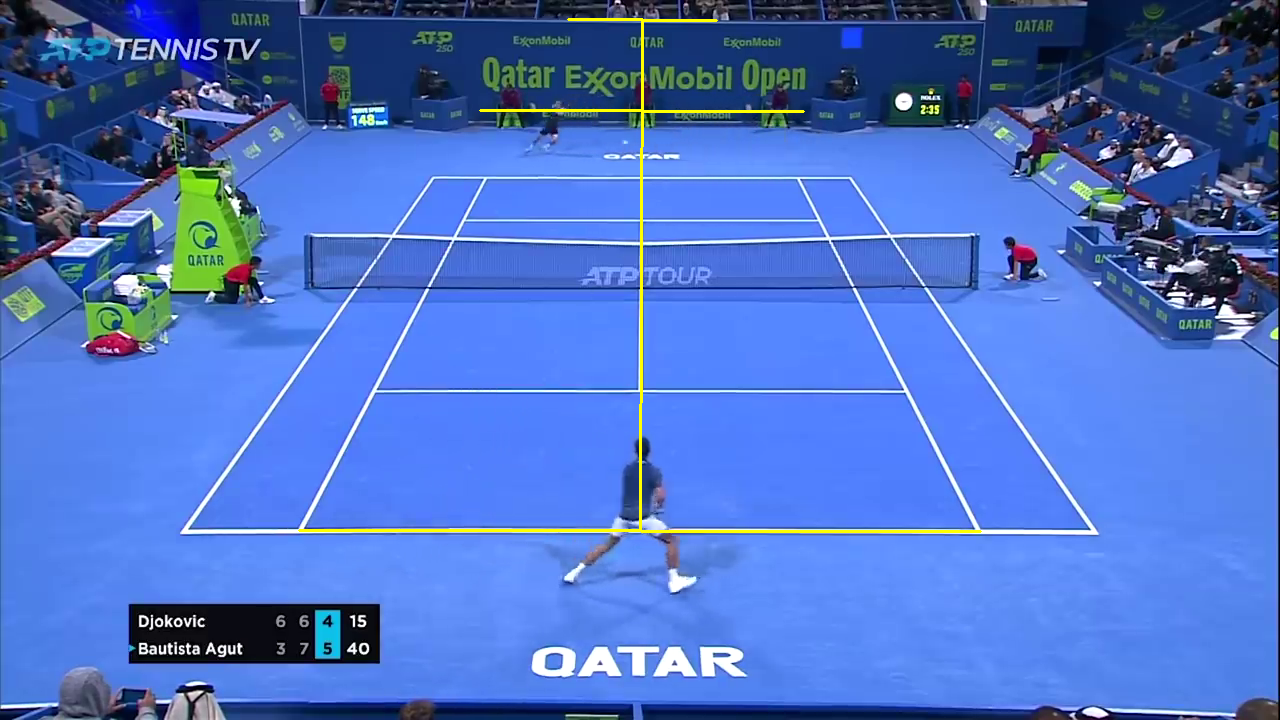
\includegraphics[width=\linewidth]{figures/generated/classical/real_outlier_overlay.png}
    \caption{実写で唯一大きな外挿を含んだ例。}
  \end{subfigure}\hfill
  \begin{subfigure}[t]{0.32\linewidth}
    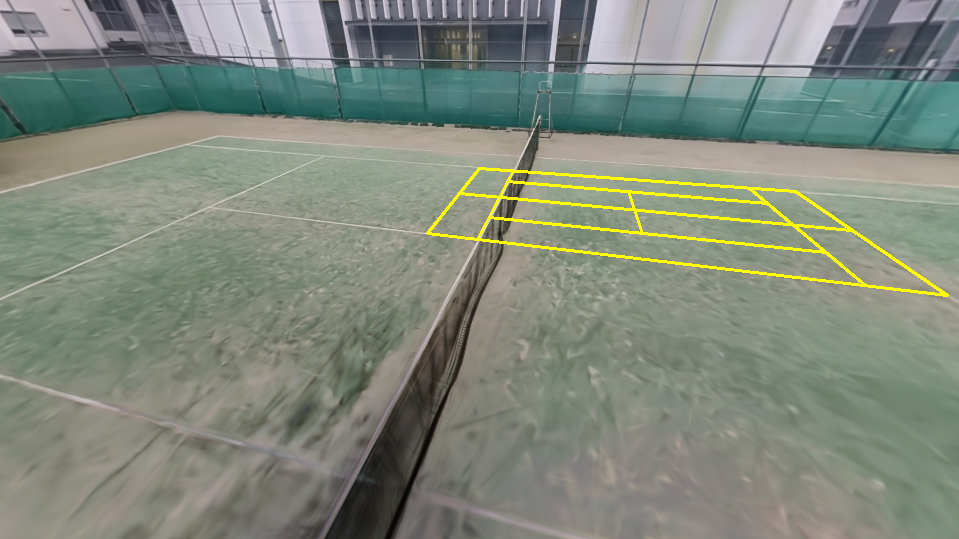
\includegraphics[width=\linewidth]{figures/generated/classical/synthetic_wrong_fit.png}
    \caption{16 点を返したが誤フィットした合成例。}
  \end{subfigure}\hfill
  \begin{subfigure}[t]{0.32\linewidth}
    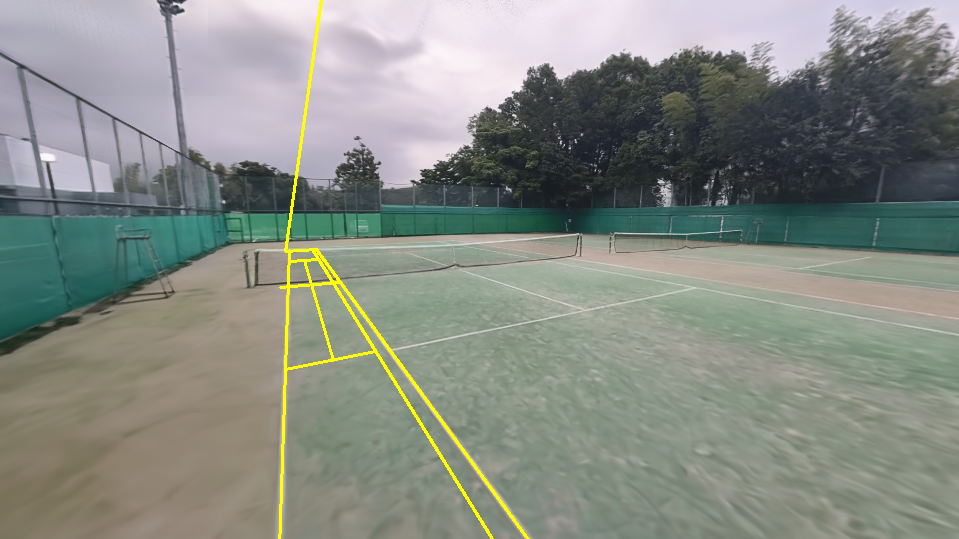
\includegraphics[width=\linewidth]{figures/generated/classical/synthetic_extreme_overlay.png}
    \caption{外接矩形がフレームの \(2.39\times56.77\) に広がった合成例。}
  \end{subfigure}
  \caption{\textbf{古典的コートモデル当てはめの補助 probe の代表例。}
  黄はこの実装が返した 16 点が作るコートモデルである。
  主比較とは別の決定論的な標本から選んだ例であり、
  主比較の数値と直接対応しない。
  }
  \label{fig:classical_probe}
\end{figure}

\begin{figure}[t]
  \centering
  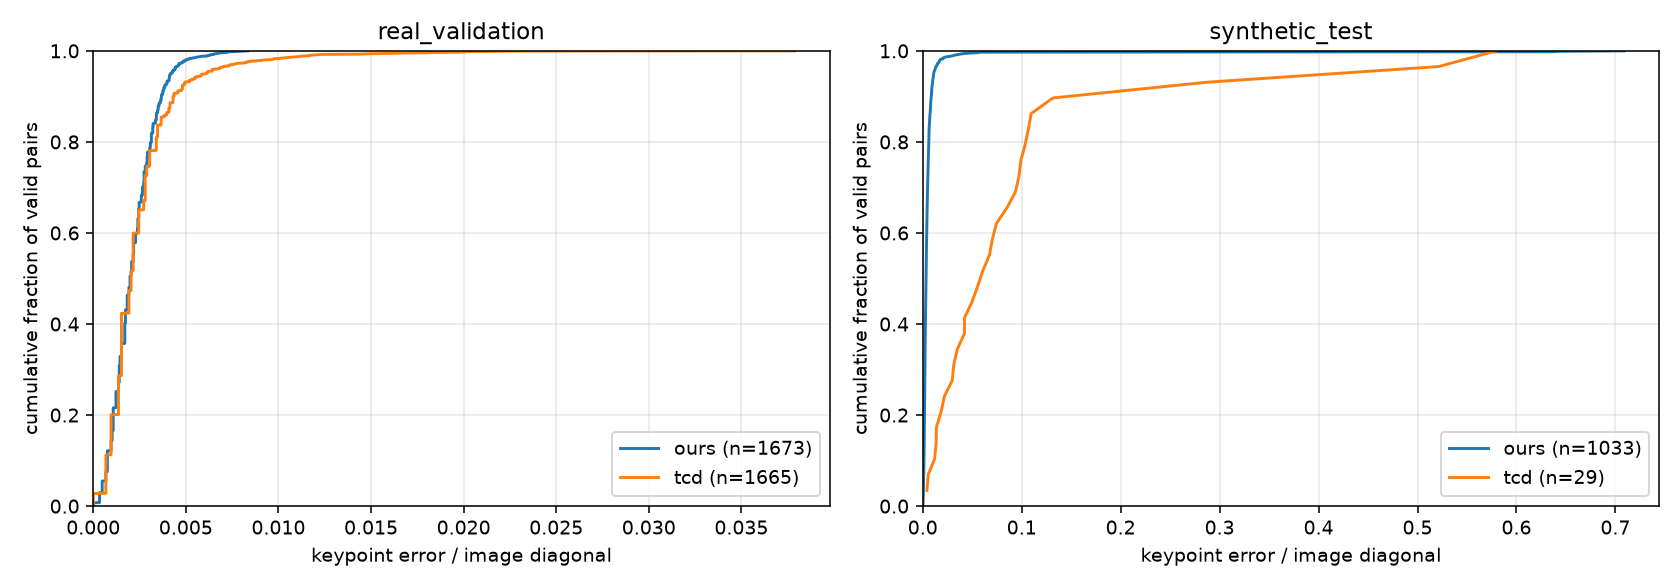
\includegraphics[width=\linewidth]{figures/generated/error_cdf.png}
  \caption{\textbf{有効対応のみのキーポイント誤差 CDF。}
  横軸は画像対角線で正規化した対応誤差、
  縦軸は有効対応の累積割合である。
  欠落したキーポイントはこの図に含まれないため、
曲線の \(n\) はモデル間で異なる
（実写 \resRealOursPairN{} 対 \resRealTcdPairN、
合成 \resSynthOursPairN{} 対 \resSynthTcdPairN）。
同一 domain 内でも曲線ごとに \(n\) が異なる点に注意する。
  }
  \label{fig:error_cdf}
\end{figure}

\subsection{checkpoint 選択時の synthetic validation}
\label{sec:ckpt_validation}

\cref{tab:ckpt_validation} に、
一つの学習 run が epoch \resCkptEpoch で記録した
合成 validation の値を示す。
これは\cref{sec:comparison_setup} の交差モデル比較とは別の結果である。

\begin{table}[t]
  \centering
  \caption{\textbf{checkpoint 選択時に記録された合成 validation の値。}
  単一 run、単一 validation、epoch \resCkptEpoch の一行である。
  同一条件の比較ベンチマークではなく、
  実写 held-out でも、複数 seed の平均でもない。
  この run は epoch 18 で停止しており、完走していない。
  }
  \label{tab:ckpt_validation}
  \small
  \begin{tabular}{@{}llr@{}}
    \toprule
    指標 & 単位 & 値 \\
    \midrule
    \KPName{} 平均距離 & px & \resCkptKPMeanPx \\
    \KPName{} 中央値距離 & px & \resCkptKPMedianPx \\
    領域分割 mIoU & --- & \resCkptSegMIoU \\
    二値線 Dice & --- & \resCkptLineDice \\
    線の意味分類 mIoU & --- & \resCkptSemanticLineMIoU \\
    姿勢再投影距離（姿勢のみ） & px & \resCkptPoseReprojectionPx \\
    カメラ中心 L2 誤差 & m & \resCkptTranslationLtwoM \\
    回転測地誤差 & 度 & \resCkptRotationGeodesicDeg \\
    焦点距離の相対誤差 & --- & \resCkptFocalRelativeError \\
    対数焦点距離の絶対誤差 & --- & \resCkptLogFocalAbsError \\
    教師有効キーポイント数（validation 合計） & 個 &
      \resCkptVisiblePointCount \\
    \bottomrule
  \end{tabular}
\end{table}


この表について、次の四つを明示する。

\begin{enumerate}[leftmargin=1.6em]
  \item これは\emph{同一条件の比較ベンチマークではない}。
  比較相手に同じデータ、同じ更新回数、同じ入力解像度を与えた測定ではない。
  \item 検証は合成側の held-out である。
  実写 held-out validation の値ではない。
  未知会場や非放送実写への汎化を示さない。
  \item validation はこの run で一度だけ記録されている。
  複数 seed の平均でも分散でもない。
  \item この run は最後まで完走していない。
  epoch 18 の 91\% で、
  破損した \texttt{byte\_planes.npy} を含む
  \texttt{npz} アーカイブの CRC 不一致により停止した。
  したがって\cref{tab:ckpt_validation} は
  \emph{完走した run の最終 epoch} の値ではない。
\end{enumerate}

来歴を隠さない理由は単純である。
停止した run の途中 checkpoint を、
完走した最良モデルとして提示すれば、
後続の比較が同じ条件で再現できなくなる。
付録~\ref{app:reproducibility} に run の同定情報と停止理由を記す。

\subsection{negative evidence の記録}
\label{sec:negative_evidence}

失敗したアライメントは、
成功例と同じ重みで記録する。
\cref{sec:holdout} で述べた B00 の校正試行はその一例である。
集約した fit 残差が閾値を満たしても、
fit のカメラ集合を 8 グループずつ三通りに選び直すと
コート中心が最大 \(9.08\) m、方位が \(89.94^\circ\) ずれ、
安定性の判定で棄却された。
続く局所再当てはめは fit を通ったが、
凍結変換の holdout は距離重み付き q95 が \(1.240\) m、
グループ別のテンプレート被覆が最小 \(0.223\) となり棄却された。
どちらの試行でも機械受理の契約は公開していない。

この記録は、\cref{eq:template_fit} の目的関数を最大化すれば
正しい変換が得られるという主張への反例である。
平均のスコアと内点率だけでは足りず、
部分集合への依存と全テンプレートの被覆を見る必要がある。
同じ理由で、\cref{sec:results_classical} の
クラッシュと縮退も削除せずに残す。
16 点を返したという事実は、
その 16 点がコートを支持していることを意味しない。
